\documentclass[preview]{standalone}
\usepackage{amsmath}
\usepackage{amssymb}
\usepackage{stellar}
\usepackage{definitions}
\usepackage{bettelini}
\usepackage{tikz}
\usepackage{pgfplots}
\pgfplotsset{compat=1.18}
\begin{document}
\id{diffeq-existence-uniqueness}
\genpage
\section{Lipschitz conditions}

\begin{snippetdefinition}{diffeq-state-lipschitz-definition}{Lipschitz continuity in the state}
    For \(f\colon\Omega\subseteq\realnumbers\times\realnumbers^m\fromto\realnumbers^m\),
    a Lipschitz bound on a cylinder \(I\times B\subseteq\Omega\) is
    \[
        \|f(t,u)-f(t,v)\|\leq L\|u-v\|
        \quad(t\in I,\ u,v\in B),
    \]
    for a constant \(L\geq0\) independent of \(t\).
    The \function is \emph{locally Lipschitz in the state, uniformly locally in time}
    if such a bound holds on a neighborhood cylinder of every point of \(\Omega\).
\end{snippetdefinition}

\begin{snippetproposition}{diffeq-continuous-state-jacobian}{A derivative criterion}
    Let \(f\colon\Omega\fromto\realnumbers^m\), with \(\Omega\) open,
    be continuous and have a continuous state Jacobian \(D_yf\).
    Then \(f\) is locally Lipschitz in the state, uniformly locally in time.
\end{snippetproposition}

\begin{snippetproof}{diffeq-continuous-state-jacobian-proof}{diffeq-continuous-state-jacobian}{A derivative criterion}
    On a compact cylinder with a convex state ball, continuity bounds
    \(\|D_yf\|\) by some \(L\). For two state points in that ball,
    \[
        f(t,u)-f(t,v)=\int_0^1D_yf(t,v+s(u-v))(u-v)\,ds.
    \]
    Taking norms gives the required uniform Lipschitz bound.
\end{snippetproof}

\begin{snippetexample}{diffeq-state-lipschitz-not-continuous}{Continuity in time is separate}
    The \function \(f(t,y)=\chi_{\rationalnumbers}(t)\) is Lipschitz in \(y\)
    with constant zero, since it is constant along every vertical line.
    Nevertheless it is discontinuous everywhere.
    State Lipschitz continuity does not replace joint continuity.
\end{snippetexample}

\begin{snippettheorem}{diffeq-peano-existence}{Peano existence theorem}
    If \(\Omega\subseteq\realnumbers^{m+1}\) is open and
    \(f\colon\Omega\fromto\realnumbers^m\) is continuous, every
    \((t_0,y_0)\in\Omega\) admits a local solution of
    \(y'=f(t,y)\), \(y(t_0)=y_0\). Uniqueness is not asserted.
\end{snippettheorem}

\section{The global Lipschitz theorem}

\begin{snippettheorem}{diffeq-global-lipschitz-existence}{Existence on a compact time interval}
    Let \(I\) be a compact interval, \(t_0\in I\), and
    \(f\in C(I\times\realnumbers^m,\realnumbers^m)\).
    Suppose \(\|f(t,u)-f(t,v)\|\leq L\|u-v\|\) for all \(t\in I\), \(u,v\in\realnumbers^m\).
    For every \(y_0\), the initial value problem \(y'=f(t,y)\), \(y(t_0)=y_0\)
    has exactly one solution in \(C^1(I,\realnumbers^m)\).
\end{snippettheorem}

\begin{snippetproof}{diffeq-global-lipschitz-existence-proof}{diffeq-global-lipschitz-existence}{Existence on a compact time interval}
    On the Banach space \(X=C(I,\realnumbers^m)\), define
    \[
        (Tu)(x)=y_0+\int_{t_0}^x f(t,u(t))\,dt,\qquad
        a=\max_{x\in I}|x-t_0|.
    \]
    Continuous integrands make \(T\colon X\fromto X\) well defined.
    Fixed points are exactly the required solutions. The immediate estimate
    \(\|Tu-Tv\|_\infty\leq La\|u-v\|_\infty\) need not make \(T\) a contraction.
    Instead we prove by induction
    \[
        \|T^ku(x)-T^kv(x)\|
        \leq\frac{L^k|x-t_0|^k}{k!}\|u-v\|_\infty.
    \]
    For \(k=1\), bound the integrand by \(L\|u-v\|_\infty\).
    Assuming the estimate for \(k\), for \(x\geq t_0\),
    \begin{align*}
        \|T^{k+1}u(x)-T^{k+1}v(x)\|
        &\leq L\int_{t_0}^x\|T^ku(t)-T^kv(t)\|\,dt\\
        &\leq\frac{L^{k+1}}{k!}\|u-v\|_\infty
             \int_{t_0}^x(t-t_0)^k\,dt\\
        &=\frac{L^{k+1}(x-t_0)^{k+1}}{(k+1)!}\|u-v\|_\infty.
    \end{align*}
    For \(x\leq t_0\), reverse the limits and obtain the same bound with
    \(|x-t_0|\). Thus
    \[
        \|T^ku-T^kv\|_\infty\leq\frac{(La)^k}{k!}\|u-v\|_\infty.
    \]
    Since \((La)^k/k!\to0\), some \(T^N\) is a contraction.
    The \snippetref[banach-fixed-point-theorem][Banach fixed-point theorem]
    gives its unique fixed point \(u\).
    Now \(T^N(Tu)=T(T^Nu)=Tu\), so uniqueness for \(T^N\) gives \(Tu=u\).
    Conversely every fixed point of \(T\) is fixed by \(T^N\); this proves uniqueness.
\end{snippetproof}

\begin{snippet}{diffeq-iteration-time-interval}
    The factorial estimate imposes no smallness restriction on the compact
    interval. In this original sketch the initial time is denoted by \(x_0\).
\begin{center}
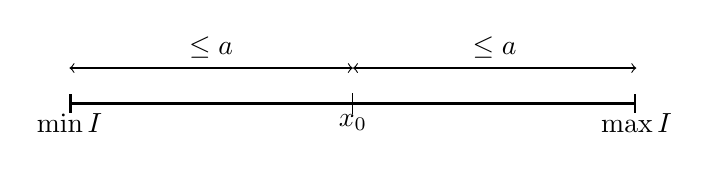
\begin{tikzpicture}[x=1.2cm,y=1cm]
	\draw[|-|,thick] (-3,0) -- (3,0);
	\draw (0,0.13) -- (0,-0.13);
	\node[below] at (-3,0) {\(\min I\)};
	\node[below] at (0,-0.02) {\(x_0\)};
	\node[below] at (3,0) {\(\max I\)};
	\draw[<->] (-3,0.45) -- (0,0.45) node[midway,above] {\(\leq a\)};
	\draw[<->] (0,0.45) -- (3,0.45) node[midway,above] {\(\leq a\)};
\end{tikzpicture}
\end{center}
\end{snippet}

\section{Local existence}

\begin{snippettheorem}{diffeq-cauchy-lipschitz-cylinder}{Cauchy--Lipschitz theorem}
    Let \(\Omega\subseteq\realnumbers^{m+1}\) be open and \(f\in C(\Omega,\realnumbers^m)\).
    Suppose \(R=[a,b]\times\overline B_r(y_0)\subseteq\Omega\),
    \(a<t_0<b\), \(r>0\), and \(f\) is Lipschitz in the state on \(R\)
    with a uniform constant \(L\). Put \(M=\max_R\|f\|\).
    The initial value problem \(y'=f(t,y)\), \(y(t_0)=y_0\) has a unique
    solution on
    \[
        J=[a,b]\cap[t_0-r/M,t_0+r/M].
    \]
    Here \(r/M=+\infty\) when \(M=0\). Its graph remains in \(R\).
\end{snippettheorem}

\begin{snippetproof}{diffeq-cauchy-lipschitz-cylinder-proof}{diffeq-cauchy-lipschitz-cylinder}{Cauchy--Lipschitz theorem}
    Replace the full function space by
    \[
        X=C(J,\overline B_r(y_0))
        =\{u\in C(J,\realnumbers^m):\|u-y_0\|_\infty\leq r\}.
    \]
    It is not a vector space, but it is a nonempty closed ball in a Banach space,
    hence a complete metric space. For the Volterra operator,
    \[
        \|Tu(x)-y_0\|
        \leq\left|\int_{t_0}^x\|f(t,u(t))\|\,dt\right|
        \leq M|x-t_0|\leq r.
    \]
    Thus \(T\) maps \(X\) into itself. The factorial estimate in the global
    proof applies without change, giving a unique fixed point.
    Any other solution starting at \(y_0\) remains inside the ball until it
    first reaches its boundary; the same speed estimate shows this cannot
    happen before time distance \(r/M\). Uniqueness therefore applies on \(J\).
    If \(M=0\), the constant \(y_0\) is the solution on all of \([a,b]\).
\end{snippetproof}

\begin{snippetproposition}{diffeq-bounded-speed-cone}{The bounded-speed estimate}
    If a solution \(y\) of \(y'=f(t,y)\) satisfies \(\|f(t,y(t))\|\leq M\)
    between \(t_0\) and \(t\), then
    \[
        \|y(t)-y(t_0)\|\leq M|t-t_0|.
    \]
    For a scalar equation its graph lies in the double cone
    \(|y-y_0|\leq M|t-t_0|\), whose half-angle from the horizontal is \(\arctan M\).
\end{snippetproposition}

\begin{snippetproof}{diffeq-bounded-speed-cone-proof}{diffeq-bounded-speed-cone}{The bounded-speed estimate}
    Integrate \(y'=f(t,y(t))\) and apply the integral triangle inequality.
    On a bounded state cylinder the cone may reach its horizontal sides,
    which explains the time restriction in the local theorem.
\end{snippetproof}

\section{Picard iteration and noncompact intervals}

\begin{snippetcorollary}{diffeq-picard-iteration-convergence}{Convergence of successive approximations}
    Under the hypotheses of the compact global Lipschitz theorem, for any
    \(u_0\in C(I,\realnumbers^m)\), the iterates \(u_{n+1}=Tu_n\) converge
    uniformly to the unique solution \(u\). The same holds on the local
    cylinder interval if \(u_0\in C(J,\overline B_r(y_0))\).
\end{snippetcorollary}

\begin{snippetproof}{diffeq-picard-iteration-convergence-proof}{diffeq-picard-iteration-convergence}{Convergence of successive approximations}
    Since \(T^nu=u\), the factorial estimate gives
    \(\|T^nu_0-u\|_\infty\leq(La)^n\|u_0-u\|_\infty/n!\to0\).
\end{snippetproof}

\begin{snippetexample}{diffeq-picard-exponential}{The exponential from iteration}
    For \(y'=y\), \(y(0)=1\), start with \(u_0=1\). Then
    \[
        u_1=1+\int_0^x1\,dt=1+x,\qquad
        u_2=1+\int_0^x(1+t)\,dt=1+x+\frac{x^2}{2}.
    \]
    Inductively \(u_n=\sum_{j=0}^n x^j/j!\to e^x\) uniformly on compact intervals.
    Any other continuous starting function also converges to \(e^x\), though
    its iterates need not be these Taylor polynomials.
\end{snippetexample}

\begin{snippetcorollary}{diffeq-global-lipschitz-open-interval}{Existence on an arbitrary time interval}
    Let \(I\) be open and \(f\in C(I\times\realnumbers^m,\realnumbers^m)\).
    If for every compact \(J\subset I\) there is \(L_J\) such that \(f\)
    is \(L_J\)-Lipschitz in \(y\) on \(J\times\realnumbers^m\), then every
    initial value problem has a unique solution on all of \(I\).
    Picard iteration converges locally uniformly in time.
\end{snippetcorollary}

\begin{snippetproof}{diffeq-global-lipschitz-open-interval-proof}{diffeq-global-lipschitz-open-interval}{Existence on an arbitrary time interval}
    Exhaust \(I\) by nested compact intervals containing the initial time.
    On each the compact theorem applies. Uniqueness makes the solutions
    agree on overlaps, so they join into one solution on \(I\).
    The iteration estimate applies on each compact separately.
\end{snippetproof}

\begin{snippetexample}{diffeq-linear-exhaustion-example}{Choosing the time component}
    For \(y'=y/x+1/(x-3)\), \(y(\pi)=27\), the coefficient domain has three
    components. The relevant one is \(I=(3,+\infty)\).
    The intervals \([3+1/n,\pi+n]\), for sufficiently large \(n\), exhaust \(I\).
    On each, the state Lipschitz constant is \(\max 1/x\);
    uniqueness joins their solutions. Convergence of iterates is guaranteed
    on compact subsets, not necessarily uniformly on the entire half-line.
\end{snippetexample}

\end{document}
